%% Cleaned Beamer file converted to Metropolis
\documentclass[english,aspectratio=169]{beamer}

% -------------------------------------------------
% Fonts and encoding
% -------------------------------------------------
\usepackage[T1]{fontenc}
\usepackage[latin9]{inputenc}
\usepackage{lmodern}
\renewcommand{\sfdefault}{lmss}
\renewcommand{\ttdefault}{lmtt}

% -------------------------------------------------
% Language and layout
% -------------------------------------------------
\usepackage{babel}
\setlength{\parskip}{\medskipamount}
\setlength{\parindent}{0pt}

% -------------------------------------------------
% Math, graphics, listings
% -------------------------------------------------
\usepackage{amssymb}
\usepackage{graphicx}
\usepackage{svg}
\usepackage{color}
\usepackage{tikz}
\usepackage{listings}
\renewcommand{\lstlistingname}{Listing}

% -------------------------------------------------
% Beamer configuration
% -------------------------------------------------
%\usetheme{CambridgeUS}

% -------------------------------------------------
% Theme: Metropolis
% -------------------------------------------------
\usetheme{metropolis}
\metroset{progressbar=frametitle,sectionpage=progressbar}

% -------------------------------------------------
% UCT Brand Colors
% -------------------------------------------------
\definecolor{UCTBlue}{HTML}{009ADA}
\definecolor{UCTDarkBlue}{HTML}{00243A}

\setbeamercolor{palette primary}{bg=UCTDarkBlue, fg=white}
\setbeamercolor{frametitle}{bg=UCTDarkBlue, fg=white}
\setbeamercolor{progress bar}{fg=UCTBlue}
\setbeamercolor{title separator}{fg=UCTBlue}
\setbeamercolor{alerted text}{fg=UCTBlue}

% -------------------------------------------------
% Custom UCT title slide
% -------------------------------------------------
\setbeamertemplate{title page}{%
  \begin{tikzpicture}[remember picture,overlay]
    % Background
    \fill[UCTBlue] (current page.south west) rectangle (current page.north east);
    % Logo
    \node[anchor=north, xshift=-4cm, yshift=-1.2cm] at (current page.north)
      {\includegraphics[height=1cm]{uct_logo_horizontal_white}};
    \node[anchor=north, xshift=4cm, yshift=0cm] at (current page.north)
      {
\includegraphics[height=3cm]{samos-logo-transparent}};      
  \end{tikzpicture}
  \vspace*{3.2cm}
  \begin{center}
    {\usebeamercolor[fg]{title}\usebeamerfont{title}\textcolor{white}{\inserttitle}}\\[0.6em]
    {\usebeamerfont{subtitle}\textcolor{white}{\insertsubtitle}}\\[1.2em]
    {\usebeamerfont{author}\textcolor{white}{\insertauthor}}\\[0.3em]
    {\usebeamerfont{institute}\textcolor{white}{\insertinstitute}}\\[0.8em]
    {\usebeamerfont{date}\textcolor{white}{\insertdate}}
  \end{center}
}

% -------------------------------------------------
% Footer logo for content slides
% -------------------------------------------------
\usepackage{tikzpagenodes}
\addtobeamertemplate{footline}{}{%
  \begin{tikzpicture}[remember picture,overlay]
    \node[anchor=south east, xshift=-1cm, yshift=0cm]
      at (current page.south east)
      {\includegraphics[height=0.5cm]{uct_logo_horizontal_blue}};
    \node[anchor=south west, xshift=0cm, yshift=-0.2cm]
      at (current page.south west)
      {
\includegraphics[height=0.7cm]{samos-logo-transparent.png}};  
  \end{tikzpicture}%
}

% -------------------------------------------------
% LyX-specific definitions (kept minimal)
% -------------------------------------------------
\makeatletter

\newcommand\makebeamertitle{\frame{\maketitle}}

\AtBeginDocument{%
  \let\origtableofcontents=\tableofcontents
  \def\tableofcontents{\@ifnextchar[{\origtableofcontents}{\gobbletableofcontents}}
  \def\gobbletableofcontents#1{\origtableofcontents}
}

\newenvironment{lyxcode}
  {\begin{list}{}{
     \setlength{\rightmargin}{\leftmargin}
     \setlength{\listparindent}{0pt}
     \setlength{\itemsep}{0pt}
     \setlength{\parsep}{0pt}
     \raggedright\normalfont\ttfamily
   }\item[]}
  {\end{list}}

\makeatother

% -------------------------------------------------
% Document
% -------------------------------------------------
\begin{document}
    \title[Core 3 ]{Day 3: Revision control systems and code writing with AI assistance}
    \author{Vichi and Mangatane}
    \institute[UCT]{Department of Oceanography\\marcello.vichi@uct.ac.za}
    \date{AOS-SAMOS}
    \maketitle

\begin{frame}{Outline}
\tableofcontents{}
\end{frame}

\section{M: Revision Control Systems (0.5 hours)}
\begin{frame}{Revision Control Systems}
\begin{columns}[t]
\column{7cm}
\begin{itemize}
\item {\small{}One does not need to be a software engineer to appreciate the importance of maintaining different revisions of various objects.
RCSs have developed in the 80's for sequential and concurrent code writing, but are now being expanded to handle multiple types of files.}{\small\par}
\item {\small{}Revision Control is not just for BIG CODES (Source Code Management), but also for routine activities, especially in a shared professional environment}{\small\par}
\item {\small{}The material in this section is adapted from \href{http://swcarpentry.github.io/git-novice/}{http://swcarpentry.github.io/git-novice/}}{\small\par}
\end{itemize}

\column{7cm}


\includegraphics[scale=0.25]{figures/GIT-comic}
\end{columns}

\end{frame}
%
\begin{frame}{The concept}
\begin{columns}[t]

\column{8cm}
\begin{itemize}
\item {\footnotesize Revision control systems (RCS) start with a base version
of the document and then record the changes you make each step of the
way. You can think of it as a recording of your progress: you can
rewind to start at the base document and play back each change you
made, eventually arriving at your more recent version}
\item \footnotesize{The terms \textbf{version} and \textbf{revision} are often used as synonyms. They have technical differences in software engineering. A version is a more generic term to indicate changes in a file or
a set of files. Technically, it is often associated with \textbf{releases}
 of a software or document (e.g. v1.2). Revision is any recorded change
or combination of changes.}
\end{itemize}
    
\column{5.5cm}
\begin{center}
\includesvg[width=0.75\columnwidth]{figures/play-changes.svg}
\par\end{center}
\begin{itemize}
\item \small{Once you think of changes as separate from the document itself,
you can think about \textquotedblleft playing back\textquotedblright{}
different sets of changes on the base document, ultimately resulting
in different versions of that document.}
\end{itemize}
\end{columns}

\end{frame}
%
\begin{frame}{Concurrent versioning, committing and merging}
\begin{columns}[t]

\column{7cm}
\begin{center}
\includesvg[width=0.4\columnwidth]{figures/versions.svg}
\par\end{center}
\begin{itemize}
\item \tiny{Two users can make independent sets of changes on the same
document. This operation creates two \textbf{concurrent} versions. A change to a file is a temporary modification in RCS: saving the file is not sufficient to acknowledge the generation of a new version. This further operation is called \textbf{committing} a version}
\item \tiny{If the changes have been done to different parts, they are
\textbf{complementary}, and you can incorporate two sets of changes into the same base document}
\item \tiny{If the changes have been done to the same section of the document
they generate a \textbf{conflict}. }
\end{itemize}

\column{7cm}
\begin{center}
\includesvg[width=0.4\columnwidth]{figures/merge.svg}
\par\end{center}
\begin{itemize}
\item {\tiny{}The operation of combining the different committed versions
is called }\textbf{\tiny{}merging}{\tiny{}. In the case of conflicts it can be a very complicated process.}{\tiny\par}
\item {\tiny{}RCS is a tool that keeps track of these changes for us, effectively storing different versions of our files. It allows us to decide which changes will be added to the next revision (each record of these changes is called a }\textbf{\tiny{}commit}{\tiny{}), and
keeps useful metadata about them (when, who, what). }{\tiny\par}
\item {\tiny{}The complete history of commits for a particular project and their metadata make up a }\textbf{\tiny{}repository}{\tiny{}. Repositories
can be }\textbf{\tiny{}distributed}{\tiny{}. They are kept in sync across different computers (or your computer and a server in the cloud),
facilitating collaboration among different people.}{\tiny\par}
\end{itemize}
\end{columns}

\end{frame}

\section{M: Hands-on tutorial - GIT and GitHub (1 hours)}
%
\begin{frame}{The GIT model: local and remote repositories}
\begin{columns}

\column{6cm}
\scriptsize{GIT is now the most used RCS, thanks to its distributed model. Git is a sophisticated software; it can be rather complex, but the basic commands and procedures are quite simple} 
\begin{itemize}
\item {\tiny{}Commit: Commits all files from the staging area to local Repository}{\tiny\par}
\item {\tiny{}Push: Pushes all the changes made in local to Remote Repository}{\tiny\par}
\item {\tiny{}Fetch: Collects the changes from Remote Repository and copies them to Local Repository but does not affect our workspace}{\tiny\par}
\item {\tiny{}Pull: Collects the changes from Remote Repository and copies them to Local Repository along with merges to the current directory
or our workspace}{\tiny\par}
\end{itemize}

\column{8cm}
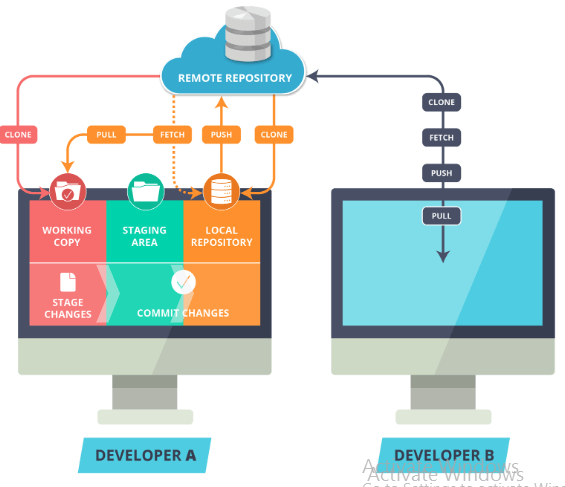
\includegraphics[width=8cm]{figures/Git-remote-local}
\end{columns}
\end{frame}

\begin{frame}{Summary of main functions}
\begin{table}
    \centering
    \begin{tabular}{|p{3.5cm}|p{9.5cm}|}
         \textbf{Term} & \textbf{Meaning} \\
\hline \hline
         Remote Repository & A server where all the collaborators upload changes made to files\\
         Local Repository & User's copy of a remote repository. It must be synchronized manually\\
         Clone Command & Creates a local copy of an existing remote repository inside a local repository\\
         Workspace copy & Users' active directory. All files (including folders) in this directory will be tracked \\
         Stage Area & It is a place where all the modified files marked to be committed are placed \\
    \end{tabular}
\end{table}

\end{frame}

%
\begin{frame}{Public services: GitHub}
\begin{columns}[t]

\column{7cm}
\begin{itemize}
\item {\footnotesize{}\href{https://github.com}{GitHub} is a web-based
Git version control repository hosting service. It provides all of
the distributed version control and source code management functionalities
of Git for collaborative projects }{\footnotesize\par}
\item {\tiny{}Git}{\tiny\par}
\begin{itemize}
\item {\tiny{}It is a software }{\tiny\par}
\item {\tiny{}It is installed locally on the system }{\tiny\par}
\item {\tiny{}It is a tool to manage different versions of files}{\tiny\par}
\item {\tiny{}It is a command-line tool (some GUIs available but not recommended)}{\tiny\par}
\end{itemize}
\item {\tiny{}GitHub}{\tiny\par}
\begin{itemize}
\item {\tiny{}It is a service }{\tiny\par}
\item {\tiny{}It is hosted on the Web }{\tiny\par}
\item {\tiny{}It is a space to upload a copy of a Git repository }{\tiny\par}
\item {\tiny{}It provides a graphical interface through the browser }{\tiny\par}
\item {\tiny{}It enables to track issues and to create a collaborative development
environment}{\tiny\par}
\end{itemize}
\end{itemize}

\column{6cm}
\begin{center}
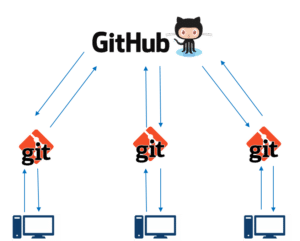
\includegraphics[scale=0.35]{figures/Github}
\par\end{center}
\begin{itemize}
\item \scriptsize{We will practice git in the classroom through Jupyter Lab. For those interested in knowing more, practice the tutorial on \href{https://swcarpentry.github.io/git-novice/}{https://swcarpentry.github.io/git-novice/}.}
\end{itemize}
\end{columns}

\end{frame}

% =================================================
\begin{frame}{Hands-on tutorial}
\textbf{\texttt{git} and GitHub} with jupyter lab. Objectives:
    \begin{itemize}
    \item  Learn how to use a RCS to keep track of code changes.
    \item Organize your directory structure and store the scripts that you have created
    \begin{enumerate}
        \item First, open an account on GitHub and learn how to create a remote repository \href{https://docs.github.com/en/get-started/start-your-journey/creating-an-account-on-github}{https://docs.github.com/en/get-started/start-your-journey/creating-an-account-on-github}
        \item  Your repository will be named SAMOS-<UCT-ID> and must be public
        \item Clone your new repository from within jupyter lab using the git integration on the left tab
        \item Create a new folder called \texttt{classroom} and move there the script that we created during Day 1 to download the sea ice data. (use a meaningful name!)
        \item commit and push the changes to the remote repository
    \end{enumerate}
    \end{itemize}
     
\end{frame}

\section{M: In-class assignment - Using LLM for coding (1 hour)}
%
\begin{frame}{In-class exercise}
    We will follow the instructions given in Exercise E2 on Amathuba.
\end{frame}
\end{document}
